\documentclass[a4paper,11pt]{scrreprt}
\include{settings/setup_koma}
% Set margins
% \usepackage{geometry}
% \geometry{
%   a4paper,
%   left=30mm,
%   top=30mm,
%   right=20mm,
%   bottom=20mm
% }
% Set document language
\usepackage[ngerman]{babel}
% Set character encoding
\usepackage[utf8]{inputenc}
% Set font enconding
\usepackage[T1]{fontenc}
% Allow usage of pictures
\usepackage{graphicx}
% Use Book-Style tables
\usepackage{booktabs}
% tabitem with bullet
\newcommand{\tabitem}{~~\llap{\textbullet}~~}
% Use modern default font
\usepackage{lmodern}
% Arial font
\renewcommand{\rmdefault}{phv}
\renewcommand{\sfdefault}{phv}
% Remove trailing dot from chapter numbering
\renewcommand{\autodot}{}
% Enable mutli-columns
\usepackage{multicol}
% Enables setting a linespacing surrounding all sections
\usepackage{setspace}
% Remove vertical seperation of items in lists
\usepackage{enumitem}
\setlist{noitemsep}
% Continuous numbering of footnotes spanning multiple chapters
\usepackage{chngcntr}
\counterwithout{footnote}{chapter}
% Change figure captions
\addto\captionsngerman{\renewcommand{\figurename}{Abb.}}
% float for pictures
\usepackage{float}
% Make ToC clickable
\usepackage[hidelinks]{hyperref}
\hypersetup{
    linktoc=all
}
% for Code listings
\usepackage{listings}
% Bibliography & Citing
\usepackage{csquotes}

% Glossary for abbreviations
\usepackage[acronym,toc]{glossaries}
\addto\captionsngerman{\renewcommand*{\acronymname}{Abkürzungsverzeichnis}}
\input{settings/setup_glossary}
% \makeglossaries  % Requires Perl to be installed
\makenoidxglossaries
\loadglsentries[acronym]{abbreviations}

% Counter to save the state of Roman numbering
\newcounter{savepage}

\begin{document}
% Cover Page 
\include{cover}

\pagenumbering{Roman}
\setcounter{page}{1}

% TOC 
\tableofcontents 
\thispagestyle{empty}

% Empty TOC page because of multi-page TOC
\addtocontents{toc}{\protect\thispagestyle{empty}}

% List of Figures
\listoffigures

% List of Abbreviations
% \printglossary[type=acronym,title=Abkürzungsverzeichnis] % Requires Perl to be installed
\printnoidxglossaries % Requires no Perl, but is slower
\clearpage

% Save Roman numbering page
\setcounter{savepage}{\arabic{page}}

% Surpress intend 
\setlength{\parindent}{0pt}
 
 
% Content
\pagenumbering{arabic}
\setcounter{page}{1}
{\setstretch{1.5}
\chapter{Einleitung} \label{chp:introduction}

\section{Projektbeschreibung} \label{sec:purpose}

Dieses Forschungsprojekt ist der erste Teil einer zweiteiligen Reihe über das Konzipieren und Entwickeln einer lokal verfügbaren \gls{restapi}. Dabei steht die Simulation eines oder mehrerer Serverendpunkte zur Abfrage von normalerweise entfernten Ressourcen im Mittelpunkt. Die Realisierung dieser Projekte erfordert die Auswahl geeigneter Technologien, die Analyse der Anforderungen sowie das Design und die Entwicklung der Software. Diese Aufgaben werden Teil des ersten Forschungsprojektes, während sich der zweite Teil der Entwicklung einer beispielhaften Software widmen könnte, welche an die im ersten Teil entwickelte \gls{restapi} angebunden wird. Das Gesamtpaket bildet schließlich eine vollständig aufeinander aufbauende Client-Server Lösung, welche ohne eine aktive Anbindung an das Internet genutzt werden kann. \\
\\ 
\section{Motivation} \label{sec:motivation}

Ein Projekt wie dieses wird zum Beispiel bei einer Präsentation benötigt, in welcher eine unzureichende Internetverbindung zu erwarten ist. So können Beispieldaten in einem Projekt wiedergegeben werden ohne auf einen entfernten Server zuzugreifen. 
Desweiteren ist in nahezu allen mittleren bis großen Unternehmen eine restriktive Internetnutzung standard. Das heißt, dass es während der Entwicklung von neuen Projekten nicht unbedingt möglich ist auf entfernte Ressourcen zuzugreifen. \cite{Hunt.1998}. Auch hier kann eine lokale \gls{restapi} sinnvoll sein, um mit Beispieldaten arbeiten zu können. 

\section{Vorgehensweise} \label{sec:approach}

Bei der Entwicklung der Software wird sich an dem Buch \textit{Software Engineering} von \textit{Ian Sommerville} orientiert \cite{Sommerville.2016}. Auf die Anforderungsanalyse wird dabei im \autoref{chp:design} eingegangen, welches ebenfalls die System- und Architekturmodellierung umfasst. Diese Ausarbeitungen werden dann im \autoref{chp:implementation} in die Praxis umgesetzt. Hier wird nun ein vollständiges Programm entwickelt, welches sowohl die \gls{api} als auch eine Benutzeroberfläche zur Anpassung der Endpunkte zur Verfügung stellt. Nach erfolgter Implementierung stellt das \autoref{chp:handbook} ein Handbuch dar, welches die Nutzung der Oberfläche und der \gls{api} illustriert. Im letzten Kapitel wird die Umsetzung überprüft und mit den Anforderungen verglichen. Ein Ausblickt gibt Aufschluss über mögliche Verbesserungen oder Erweiterungen. 
\chapter{Entwurf} \label{chp:design}

\section{Anforderungsanalyse} \label{sec:requirements} Die Anforderungsanalyse 
eines Systems oder Programms besteht aus den Beschreibungen der zu leistenden Funktionen und 
den bestehenden Beschränkungen, welchen das System unterliegt.
Dabei wird in \textit{Benutzeranforderungen} und \textit{Systemanforderungen} unterschieden. 
Ersteres wird dabei in Diagrammen und Listen dargestellt, während letzteres eine detailliertere Beschreibung der Software-Funktionen umfasst \cite{Sommerville.2016}. In diesem Zusammenhang werden zunächst grobe Anforderungen gesammelt, um anschließend eine genauere Beschreibung darzulegen. \\
Die Anforderungen werden zudem in funktionale und nicht-funktionale Anforderungen unterteilt \cite{Sommerville.2016}:

\begin{itemize}
    \item \textit{Funtionale Anforderungen} stehen für das Verhalten der Software auf zum Beispiel Benutzereingaben oder in diesem Fall Abfragen an einen Server 
    \item \textit{Nicht-funtionale Anforderungen} sind beispielsweise Beschränkungen, welche durch bestehende Standards entstehen. 
\end{itemize}

Daraus lässt sich schließen, dass funktionale Anforderungen direkt mit der Funktion des Systems in Verbindung gebracht werden können, während nicht funktionale Anforderungen die technischen Einschränkungen beschreiben. Die folgende Tabelle illustriert die Benutzeranforderungen und teilt sie in die aufgezeigten Sparten ein:

\begin{table}[ht]
    \begin{tabular}{@{}ll@{}}
    \toprule
    \textbf{Funktional} & \textbf{Nicht-funktional} \\ 
        \midrule
    \begin{tabular}[c]{@{}l@{}}Oberfläche zur konfiguration der \gls{restapi}\\
            \tabitem Manuelles Hinzufügen von Ressourcen \\
            \tabitem Hinzufügen von Ressourcen durch \\ \gls{csv} Datei\\
            \tabitem Visuelle Darstellung der Endpunkte \\
    \end{tabular} & 
    \begin{tabular}[c]{@{}l@{}}
        Betriebssystemunabhängiges Ausführen\\ 
        der Software
    \end{tabular} \\ 
        \midrule
        Persistente Datenspeicherung 
        & Operiert ohne Internetverbindung \\ 
        \midrule
        & \textit{REST}-Konform\\ 
        \bottomrule
    \end{tabular}
    \caption{Benutzeranforderungen}
\end{table}

\newpage

\subsection*{Systemanforderungen} \label{subsec:systemrequirements}
Das System muss auf den bekannten Betriebssystemen \textit{Windows}, \textit{Mac OS} sowie \textit{Linux} lauffähig sein und ohne Internetverbindung gestartet, genutzt und konfiguriert werden können. Das Starten des Programms soll einen Server starten, welcher die \gls{api} und die Benutzeroberfläche bereitstellt. Des Weiteren muss das System \gls{rest}-Komform sein. Dies bedeutet, es unterliegt einer Reihe von inoffiziellen Regeln bzw. \textit{Best-Practises}, welche im Folgenden aufgelistet werden \cite{Masse.2012}:

\paragraph{Request Methoden} 
Abfragen oder auch \textit{Requests} werden ebenfalls normgerecht verwendet. Es gibt gewisse Semantiken, die hier Verwendung finden und nach dem \gls{crud} Prinzip auf die \gls{restapi} angewendet werden.  \cite{nwg.1999} \cite{Masse.2012}:

\begin{itemize}
    \item \textbf{GET} Anzeigen von Ressourcen; wobei ohne Parameter alle Einträge abgerufen werden. (Read) \\
    Beispiel: \textit{GET http://api.localhost/studenten} \\
    Beispiel: \textit{GET http://api.localhost/studenten?id=1}
    \item \textbf{DELETE} Entfernen einer Ressource (Delete) \\
    Beispiel: \textit{DELETE http://api.localhost/studenten?id=1}
    \item \textbf{PUT/POST} Hinzufügen/Ändern einer Ressource (Create, Update) \\
    Beispiel: \textit{PUT http://api.localhost/studenten} \\
    Beispiel: \textit{POST http://api.localhost/studenten?id=1} \\
    \gls{json} formatierter Anfragebody: 
    \begin{verbatim}
        {
            name: "Jordan",
            last_name: "Riley",
            age: "23",
            subject: "Wirtschaftsinformatik"
        }
    \end{verbatim}
\end{itemize}

\paragraph{URI Format}
Generell sollte das \gls{uri} Format, welches den Pfad zum Zugriff auf eine Ressource darstellt verwendet werden. Dieser wurde 2005 unter dem Standard \textit{RFC 3986} von der \textit{Network Working Group} definiert \cite{nwg.2005}:
\begin{verbatim}
    URI = scheme "://" authority "/" path [ "?" query ] [ "#" fragment ]
\end{verbatim}
Es gibt eine Reihe von Regeln, welche bei der Konzeption einer \gls{restapi} bedacht werden sollten \cite{Masse.2012}:
\begin{itemize}
    \item \textbf{Vorwärts Slash (/)} indiziert hierarchische Ebenen. \\
    Beispiel: \textit{http://api.localhost/personen/studenten}
    \item \textbf{Kein angestelltes Slash} wird am Ende eines \gls{uri} verwendet. \\ 
    Beispiel: \textit{http://api.localhost/studenten/}
    \item \textbf{Bindestriche} werden zur Lesbarkeit verwendet.\\
    Beispiel: \textit{http://api.localhost/personen/studenten-mit-abschluss}
    \item \textbf{Dateiendungen} sind nicht mit einzuschließen. \\
    Beispiel: \textit{http://api.localhost/dokumente/lehrplan.pdf}
    \item \textbf{Suchanfragen} werden nicht in den \gls{uri} mit einbezogen, sondern dem \gls{http}-Standard gemäß übergeben.\\
    Beispiel (Falsch): \textit{http://api.localhost/studenten/getById/2} \\
    Beispiel (Richtig): \textit{http://api.localhost/studenten?id=2}
\end{itemize}

\paragraph{Status Codes} \gls{http} Status Codes informieren den Client über das Ergebnis der eingangs gestellten Abfrage. \cite{nwg.1999} Diese sind ebenfalls semantisch korrekt auf die \gls{restapi} anzuwenden:

\begin{itemize}
    \item \textbf{200 OK} ist ein allgemeiner Code, welcher über eine erfolgreiche Abfrage informiert.
    \item \textbf{201 CREATED} informiert über die erfolgreiche Erstellung einer Ressource.
    \item \textbf{404 NOT FOUND} gibt Auskunft über nicht zur Verfügung stehende Ressourcen.
    \item \textbf{500 INTERNAL SERVER ERROR} sagt aus, das ein serverseitiger Fehler aufgetreten ist.
\end{itemize}

\paragraph{CSV Datei} Neben den Anforderungen an die \gls{restapi}, ist es von Bedeutung festzulegen, in welchem Format die \gls{csv}-Datei sein sollte, um vom Server akzeptiert zu werden. Dem Standard RFC 4180 zufolge, werden verschiedene Werte durch Kommata getrennt. Reihen hingegen werden durch einen Zeilenumbruch voneinander separiert: \gls{crlf}. Die erste Zeile der Datei bildet die Kopfdaten oder auch Spaltennamen \cite{nwg.csv.1999}.

\begin{verbatim}
        field_name,field_name,field_name CRLF
        aaa,bbb,ccc CRLF
        zzz,yyy,xxx CRLF
\end{verbatim}


\section{Systemmodellierung} \label{sec:systemmodeling}
Die Systemmodellierung befasst sich primär mit der Überführung der Anforderungen in abstrakte Modelle. In diesem Kapitel wird analysiert, wie sich das System auf bestimmte Benutzereingaben verhält und welche Anwendungsszenarien zur Verfügung stehen. Dies wird Anhand von Use-Case- und Sequenzdiagrammen aufgezeigt. \cite{Sommerville.2016}

\paragraph{Verhaltensanalyse} In diesem Szenario besteht das System aus drei \textit{Teilnehmern}; dem Server \textit{(Backend)}, der Konfigurationsoberfläche (\textit{Frontend}) und dem Anwender (\textit{User}). Im ersten Fall wird dargestellt, welche Aktionen mit dem Hinzufügen von Ressourcen einhergehen (\autoref{fig:add-ressources}). Zunächst ist es dem Anwender möglich eine CSV-Datei hochzuladen oder eine Tabelle mit Daten manuell zu erstellen. Nach dem Bestätigen, werden die in der Tabelle enthaltenen Daten an den Server übertragen. Dieser legt seinerseit eine Datenbanktabelle mit entsprechenden Namen, Spalten und Spaltendaten an. Auch die \gls{api}-Endpunkte werden in einer entsprechenden Konfigurationsdatei festgelegt. Dabei werden alle in \autoref{subsec:systemrequirements} Methoden (GET, PUT/POST, DELETE) implementiert, um das Manipulieren der Daten im Anschluss zu ermöglichen. Nach erfolgreicher Erstellung wird das Frontend informiert. Dieses wiederum aktualisiert die Anzeige und stellt dem Anwender die API-Endpunkte grafisch dar.

\begin{figure}[h]
    \centering
    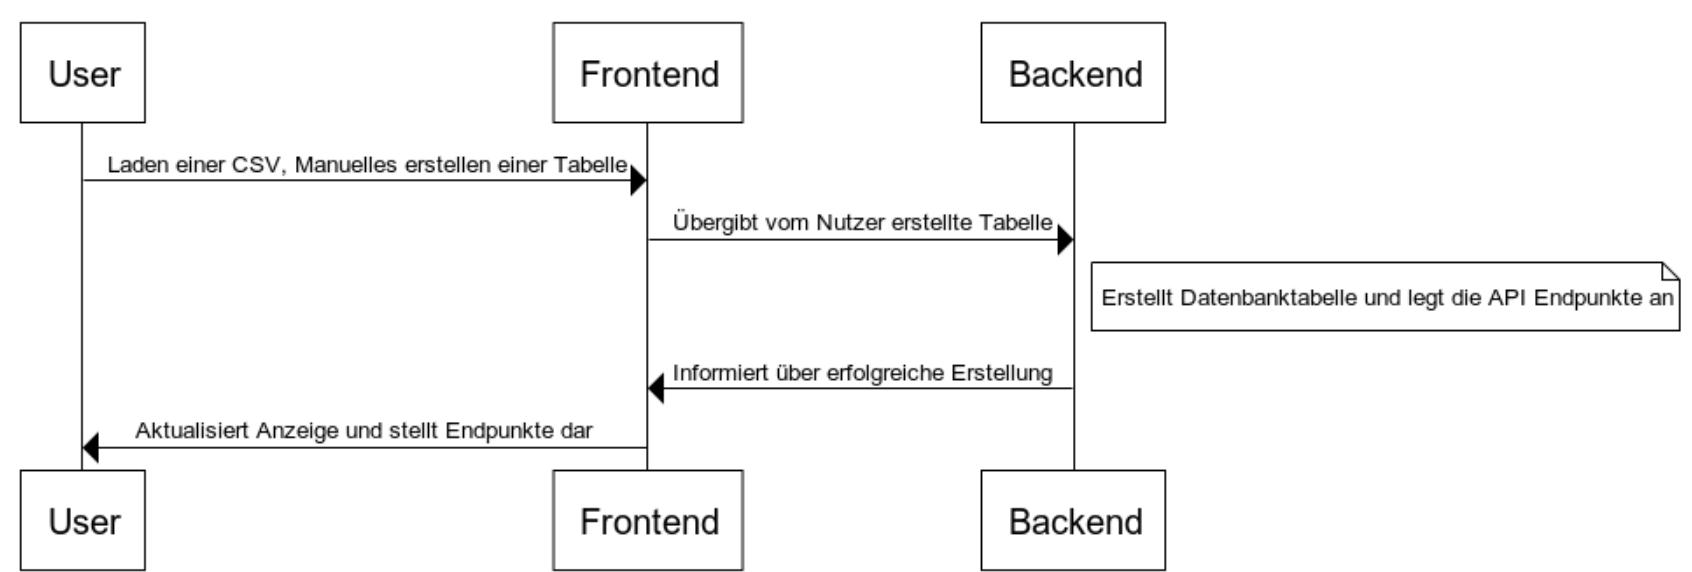
\includegraphics[width=1\textwidth]{figures/seq-hinzufuegen-von-ressourcen.png}
    \caption{Hinzufügen von Ressourcen}
    \label{fig:add-ressources}
\end{figure}

Das zweite Szenario bezieht sich auf die Abfrage einer Ressource. Zunächst wird hierbei eine \textit{GET}-Abfrage an den Server gestellt.

\begin{verbatim}
    GET http://localhost:3000/api/users?id=1
\end{verbatim}

Erwartungsgemäß sollte die Antwort des Servers ein \gls{json}-Objekt sein, welches die gespeicherten Daten des Users mit der ID 1 enthält. Nach dem Eingang der Anfrage prüft das Backend zunächst, ob die Ressource vorhanden ist. Ist dies nicht der Fall, antwortet der Server mit dem HTTP Status-Code \textit{404 NOT FOUND}. Dies indiziert das nicht vorhandensein einer angefragten Ressource. Ist sie jedoch vorhanden, ruft der Server die zugrundeliegenden Daten aus der Datenbank ab und gibt eine entsprechende \gls{json}-formatierte Nachricht zurück. Darin enthalten sind mehrere Attribute. Der Status, eine Nachricht (message), in der auch eventuelle Fehlermeldungen an den Client zurückgegeben werden können und die eigentlichen Daten (data).

\begin{figure}[h]
    \centering
    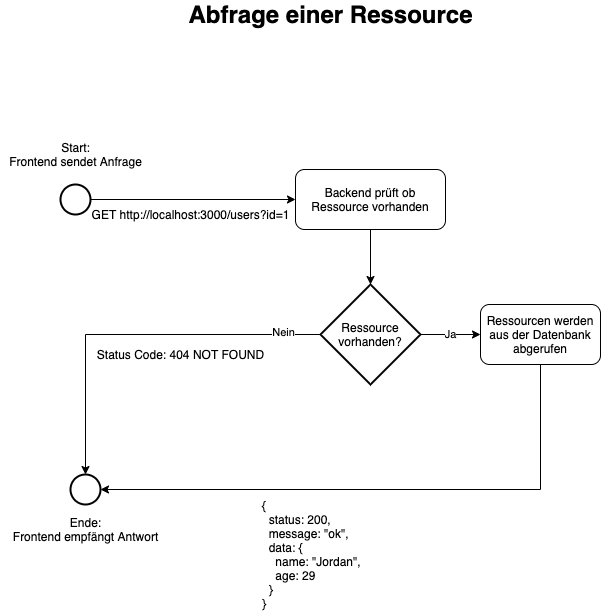
\includegraphics[width=0.8\textwidth]{figures/fc-abfrage-ressource.png}
    \caption{Abfrage einer Ressource}
    \label{fig:request-ressource}
\end{figure}
 
Daraus lässt sich also schließen, dass der Anwender auf der Konfigurationsoberfläche die Möglichkeit hat Daten entweder manuell in eine Tabelle einzutragen oder eine eigens erstellte \gls{csv}-Datei hochzuladen.
\\
Das Frontend muss mit dem Backend kommunizieren, um Tabellen anzulegen oder zu entfernen. Dies wird über eigene Endpunkte zur Administration geschehen. 

\begin{verbatim}
    PUT http://localhost:3000/api/admin/table
    DELETE http://localhost:3000/api/admin/table?name=users
\end{verbatim}

Über den \textit{PUT}-Request können Tabellen neu hinzugefügt oder überschrieben werden. Über den \textit{DELETE}-Request werden Tabellen hingegen gelöscht.
Ferner müssen Endpunkte zur Manipulation der Daten bereitgestellt werden. Da diese immer einheitlich sind, genügt es die Tabellennamen in einer Datenbank zu speichern und somit auf Validität der Endpunkte bei Abfragen zu prüfen.

\section{Architekturdesign} \label{sec:architecture}
Dieses Kapitel befasst sich zunächst mit dem groben Aufbau der Anwendung. Hierbei wird skizziert, wie Frontend, Backend und Datenbank in Relation zueinander stehen. Der zweite Teil dieses Kapitels befasst sich mit der verwendeten Technologie zur Programmierung des Frontends, Backends und der verwendeten Datenspeicherungsmethode.  

\begin{figure}[h]
    \centering
    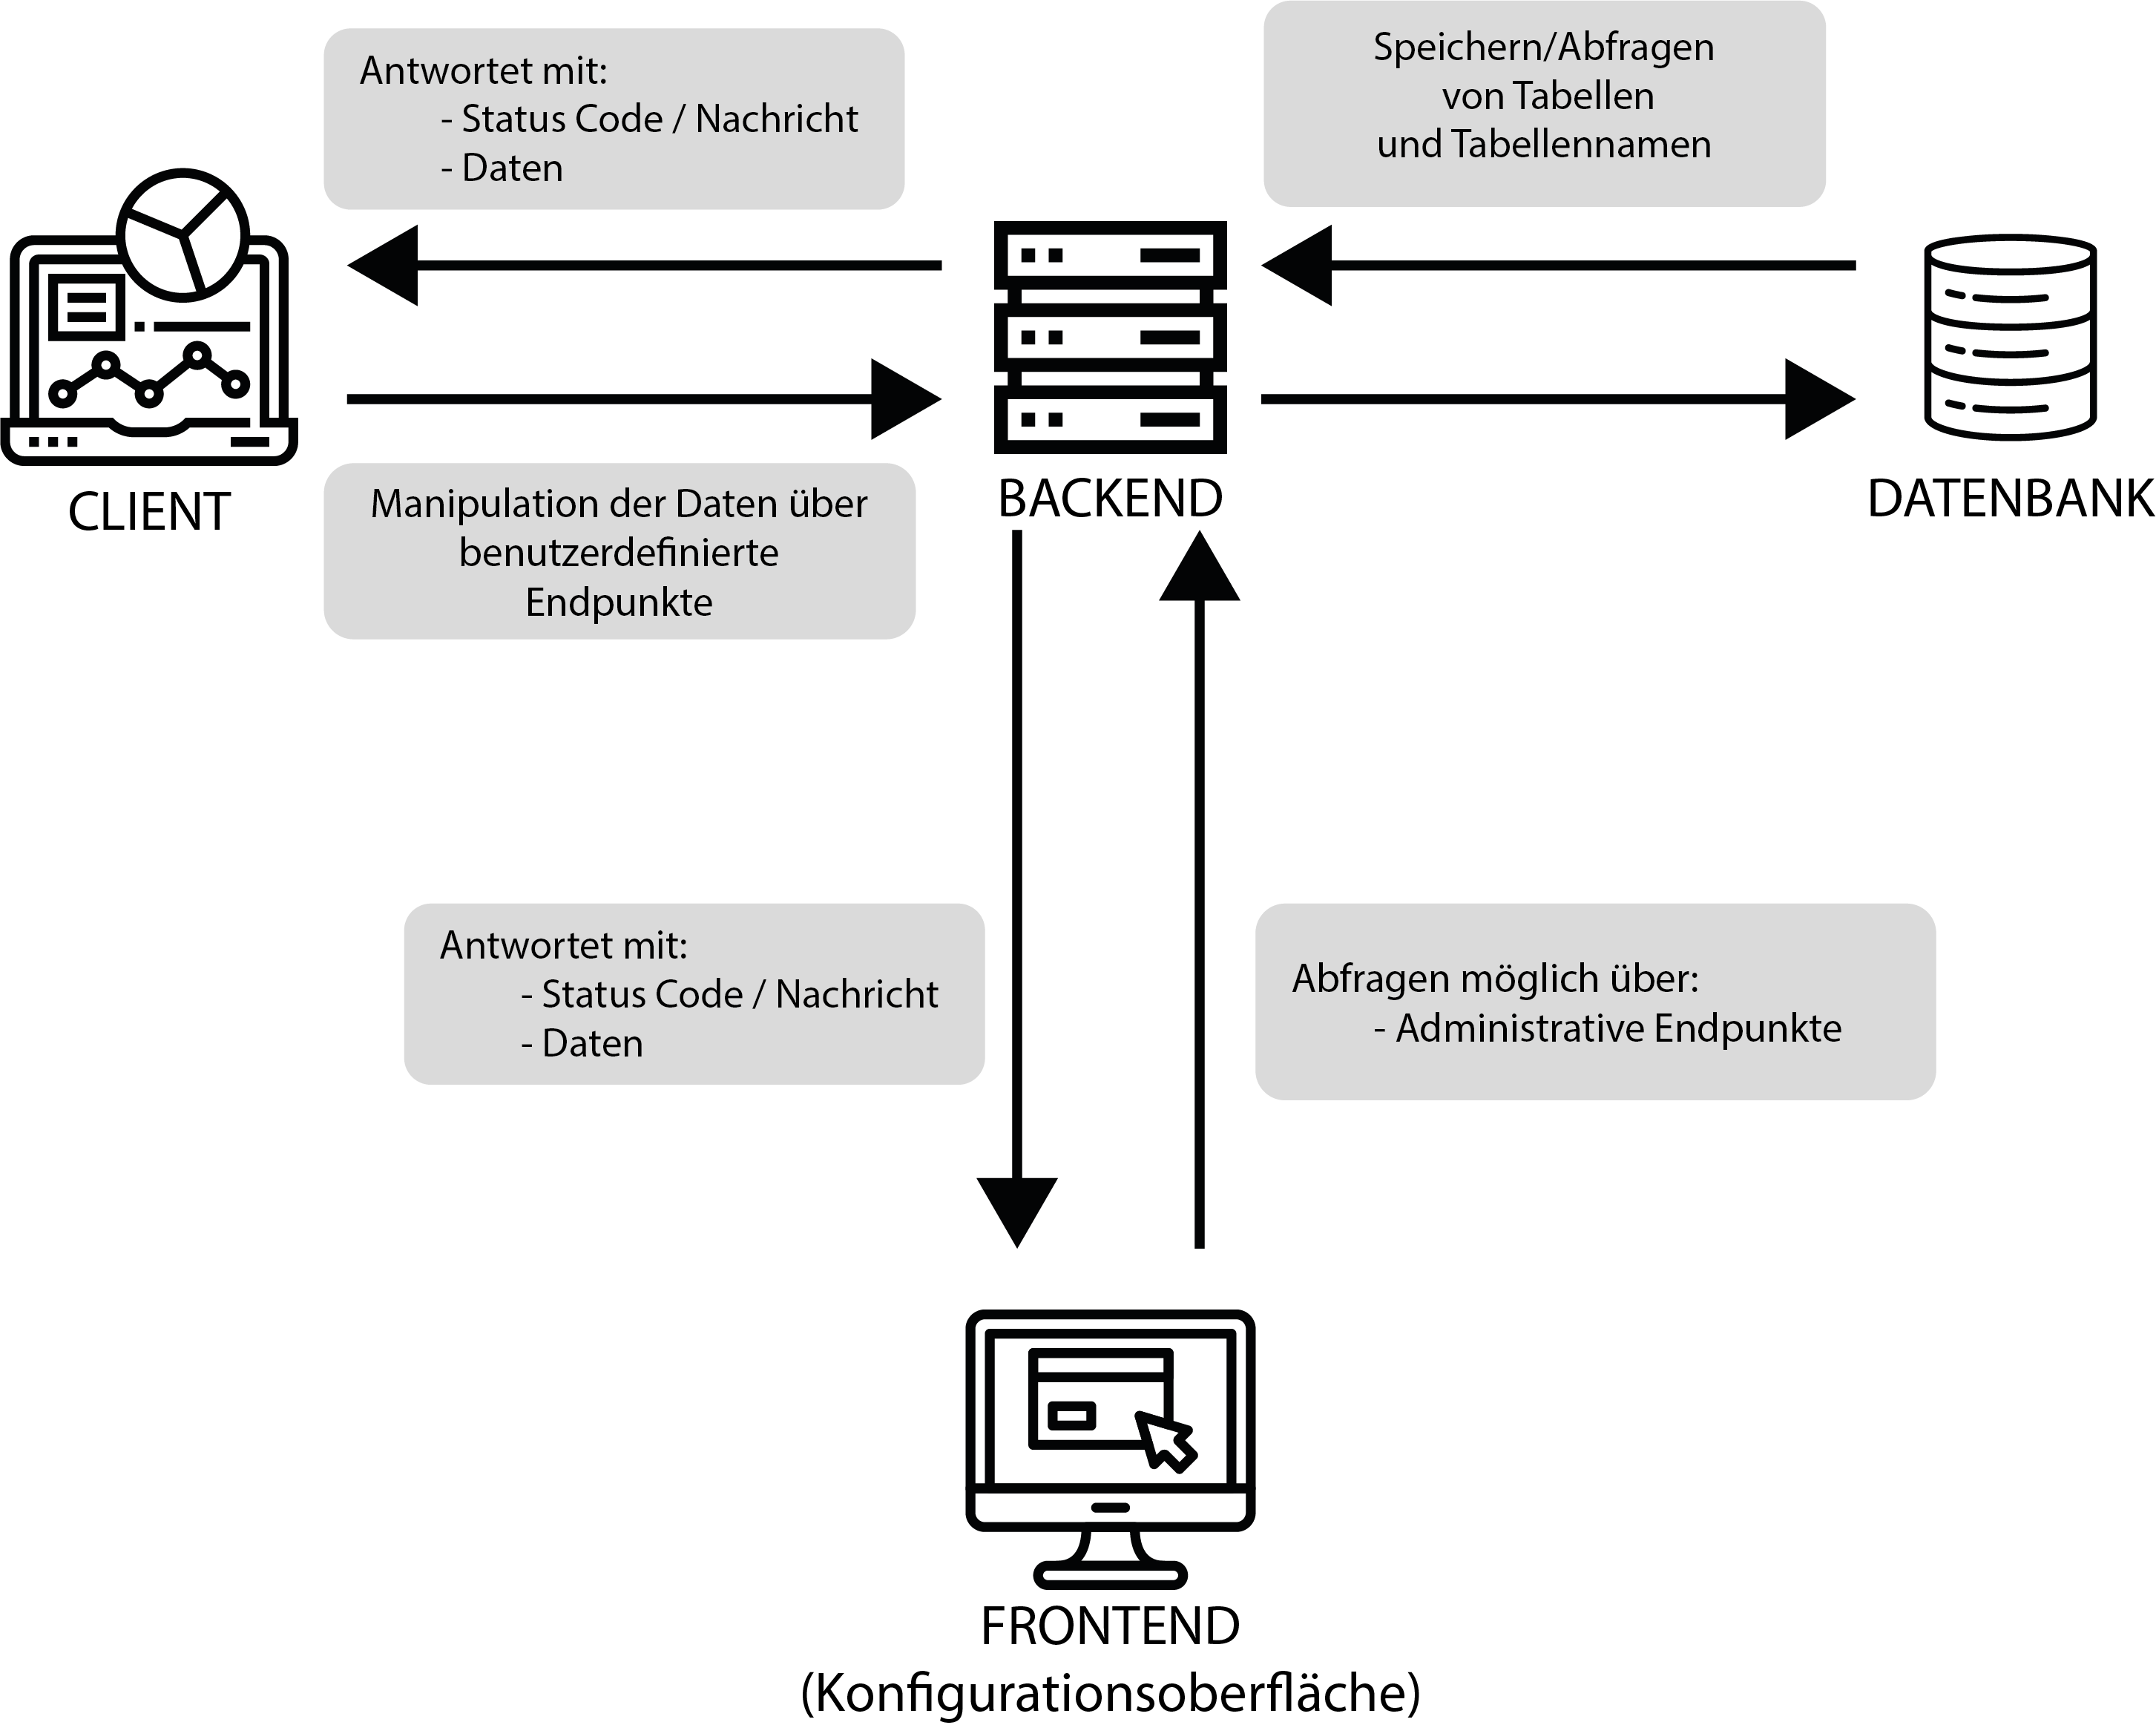
\includegraphics[width=0.8\textwidth]{figures/grobkonzept.png}
    \caption{Grobkonzept}
    \label{fig:grobkonzept}
\end{figure}

\subsubsection{Grober Entwurf}
Der erste Entwurf des Aufbaus (\autoref{fig:grobkonzept} - Icons von Flaticon\footnote{https://www.freepikcompany.com/legal}) ist in vier Teile unterteilt: Backend, Frontend, Client, Datenbank. Der Server (Backend) bildet dabei die zentrale Vermittlungsstelle. Hier werden eingehende Anfragen von der Konfigurationsoberfläche und dem Client (\gls{restapi} Nutzer) bearbeitet und beantwortet. Des Weiteren agiert der Server mit einer Datenbank, um neue Tabellen zu speichern, bestehende zu überschreiben oder zu löschen . 

\subsubsection{Verwendete Technologien}
Zur Entwicklung des gesamten Projekts müssen in diesem Abschnitt die richtigen Technologien ausgewählt werden. Dazugehören die beispielsweise  Programmiersprachen des Frontends und des Backends. Um die persistente Datenspeicherung zu ermöglichen, wird auch eine geeignete Datenbank ausgewählt. \\
Klassische Lösungen basieren auf dem sogenannten \gls{lamp}-Stack. Hierbei müsste lokal ein Apache-Server\footnote{https://httpd.apache.org/} gestartet werden, welcher PHP-Dateien\footnote{https://www.php.net/manual/de/intro-whatis.php} bereitstellt. Diese wiederum können mit einer MySQL\footnote{https://dev.mysql.com/doc/refman/8.0/en/what-is-mysql.html} Datenbank kommunizieren und die benötigten Daten bereitstellen. Zur Gestaltung der Webseiten kommen \gls{html} und \gls{css} zum Einsatz. Während \gls{html} die reine Auszeichnungssprache ist und das Grundgerüst von Komponenten darstellt, welche innerhalb des Browsers erzeugt werden, ist letzteres eine Sprache, um die Komponenten in zum Beispiel Farbe und Form zu gestalten. Die funktionale Programmiersprache \textit{JavaScript} wird hier nur dazu verwendet, um Webseiten dynamischer zu gestalten. So ist beispielsweise das Auslesen von Eingabefeldern oder das Auswerten eines Knopfdrucks möglich \cite{Gerner.2006}. \\ \\ Die Programmiersprache JavaScript hat sich im laufe der Zeit sehr weit entwickelt und findet heutzutage auch außerhalb der Browserumgebung Verwendung. Die Sprache wird beispielsweise auch Serverseitig eingesetzt und durch eine Laufzeitumgebung wie \textit{node.js}\footnote{https://nodejs.org/en/about/} für serverseitige Anwendungsszenarien eingesetzt. \cite{Resig.2016} Gleichzeitig ließe sich die Konfigurationsoberfläche ebenfalls mit node.js bereitstellen. Der Vorteil Front- und Backend in einer gemeinsamen Sprache zu programmieren legt nahe node.js für dieses Projekt einzusetzen. \\ Offen bleibt die Frage, wie Daten innerhalb des Systems persistiert werden. Wie bereits erwähnt, ist eine Möglichkeit die Nutzung einer relationalen \textit{MySQL} Datenbank. Jedoch wird hierfür ein weiterer ressourcen-intensiver Server benötigt \cite{Gerner.2006}. Für einen solchen, eher kleinen Datenbestand, lässt sich eine \textit{SQLite}-Datenbank in Betracht ziehen. Im Gegensatz zur herkömmlichen MySQL-Datenbank, werden Daten in einer Datei abgelegt und zur Laufzeit aus dieser gelesen respektive geschrieben. Trotz der serverlosen Datenbankarchitektur ermöglicht SQLite die meisten Features, welche MySQL bietet \footnote{https://www.sqlite.org/about.html}. 

\subsubsection{Systemarchitektur} \label{subsub:system-architectuere}
Ein nicht von der Hand zu weisender Faktor bei der Entwicklung von Softwareprojekten, ist der zugrunde liegende Aufbau einer Software. Bei modernen Webanwendungen wird auf das sehr weit verbreitete \gls{mvc} Muster zurückgegriffen. Dabei wird das System in mehrere Schichten unterteilt, welche verschiedene Bereiche voneinander trennen. Bei einer in node.js geschriebenen \gls{restapi} sind das typischerweise:

\begin{itemize}
    \item Model: Datenmodell; Zugriff auf Datenbank (Lesen, Schreiben); Umwandlung in JS-Objekte
    \item Controller: Verarbeiten, validieren und beantworten der eingeheneden \gls{http}-Anfragen.
    \item  Service: Business-Logik, hier ist der logische Programmcode implementiert
    \item Tests: Modultests, um einzelne Bereiche zu testen. 
    \item Sonstige: util - gemeinsame Funktionen; constants - gemeinsame Konstanten
\end{itemize}

In \autoref{fig:project-structure} ist der Aufbau des Projekts im Detail erkennbar. Der Ordner \textit{node{\_}modules} beinhaltet lediglich Module, welche von node.js genutzt werden. 
Die Konfigurationsoberfläche (View) ist ebenfalls in dieser Struktur, in Form des \textit{Public}-Ordners, vorhanden. Der Aufbau des Frontend-Ordners ist ebenfalls Modular unterteilt. So befindet sich \gls{css} in dem dafür angelegten Ordner. \textit{Assets}, also Bilddatein, Schriftarten oder sonstige Dateien, werden im gleichnamigen Ordner abgelegt. Die JavaScript-Dateien befinden sich ebenfalls in einem Unterordner. \\
Dank der Einführung von JavaScript-Modulen im Browser mit dem Standard \textit{ECMA-Script 2016} wird hier auch ein modularer Aufbau ermöglicht. Im Gegensatz zum normalen Webseiten Aufbau, kann in die Webseite ein einziges Modul importiert werden ( \textit{main.js} ), welches auf Funktionen in den einzelnen Untermodulen zugreift. Dies ermöglicht einen strukturierten und lesbareren Aufbau. \cite{Mozilla.2020}

\begin{figure}[h]
    \centering
    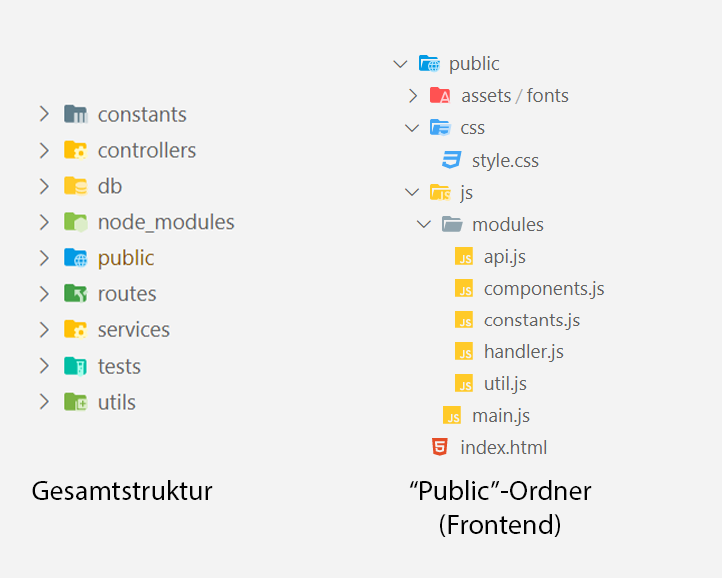
\includegraphics[width=0.6\textwidth]{figures/ordner-strukturen.png}
    \caption{Projektstruktur}
    \label{fig:project-structure}
\end{figure}

\chapter{Implementierung} \label{chp:implementation}

\section{Design Prototyp}
Um der Konfigurationsoberfläche ein Aussehen verleihen zu können, wird zunächst ein Design-Prototyp erstellt. Hierzu werden alle Komponenten aufgelistet, welche in diesem Projekt Verwendung finden.

\begin{itemize}
    \item Titelleiste mit Menüunterpunkt zum Hinzufügen neuer Endpunkte
    \item Aufklappbare Endpunktliste. Beim Aufklappen sollen Informationen zum Endpunkte ersichtlich sein.
    \item Neuer-Endpunkt/Endpunkt bearbeiten Dialog
\end{itemize}

Der erste Prototyp wird mit Adobe Illustrator\footnote{https://www.adobe.com/de/products/illustrator.html} erstellt. Das Design, wird absichtlich schlicht und übersichtlich gehalten.

Im oberen Teil lässt sich die Titelleiste erkennen, welche auch als Menü fungiert. So lässt sich mit dem Klick auf den rechten Menüpunkt zum Beispiel ein Fenster öffnen. Hier kann dann ein neuer Endpunkt manuell erstellt oder mittels \gls{csv}-Datei angelegt werden. Nach erfolgreichem Anlegen eines neuen Endpunkts erscheint dieser wiederrum in der Liste im Hauptmenü. Diese Einträge lassen sich ausklappen, sodass sichtbar wird, wie diese Endpunkte zu verwenden sind. Entsprechende \gls{http}-Methoden werden hier ersichtlich sein. Zusätzlich wären in diesem Teil auch noch weitere Bedienelemente denkbar, welche das Löschen oder Anzeigen der Endpunkte ermöglicht.

Die Anzeige der Endpunkte kann zum Beispiel in Tabellenform erfolgen. Die konkrete Implementierung wird im Kapitel \ref{sec:frontend} illustriert.

\begin{figure}[h]
    \centering
    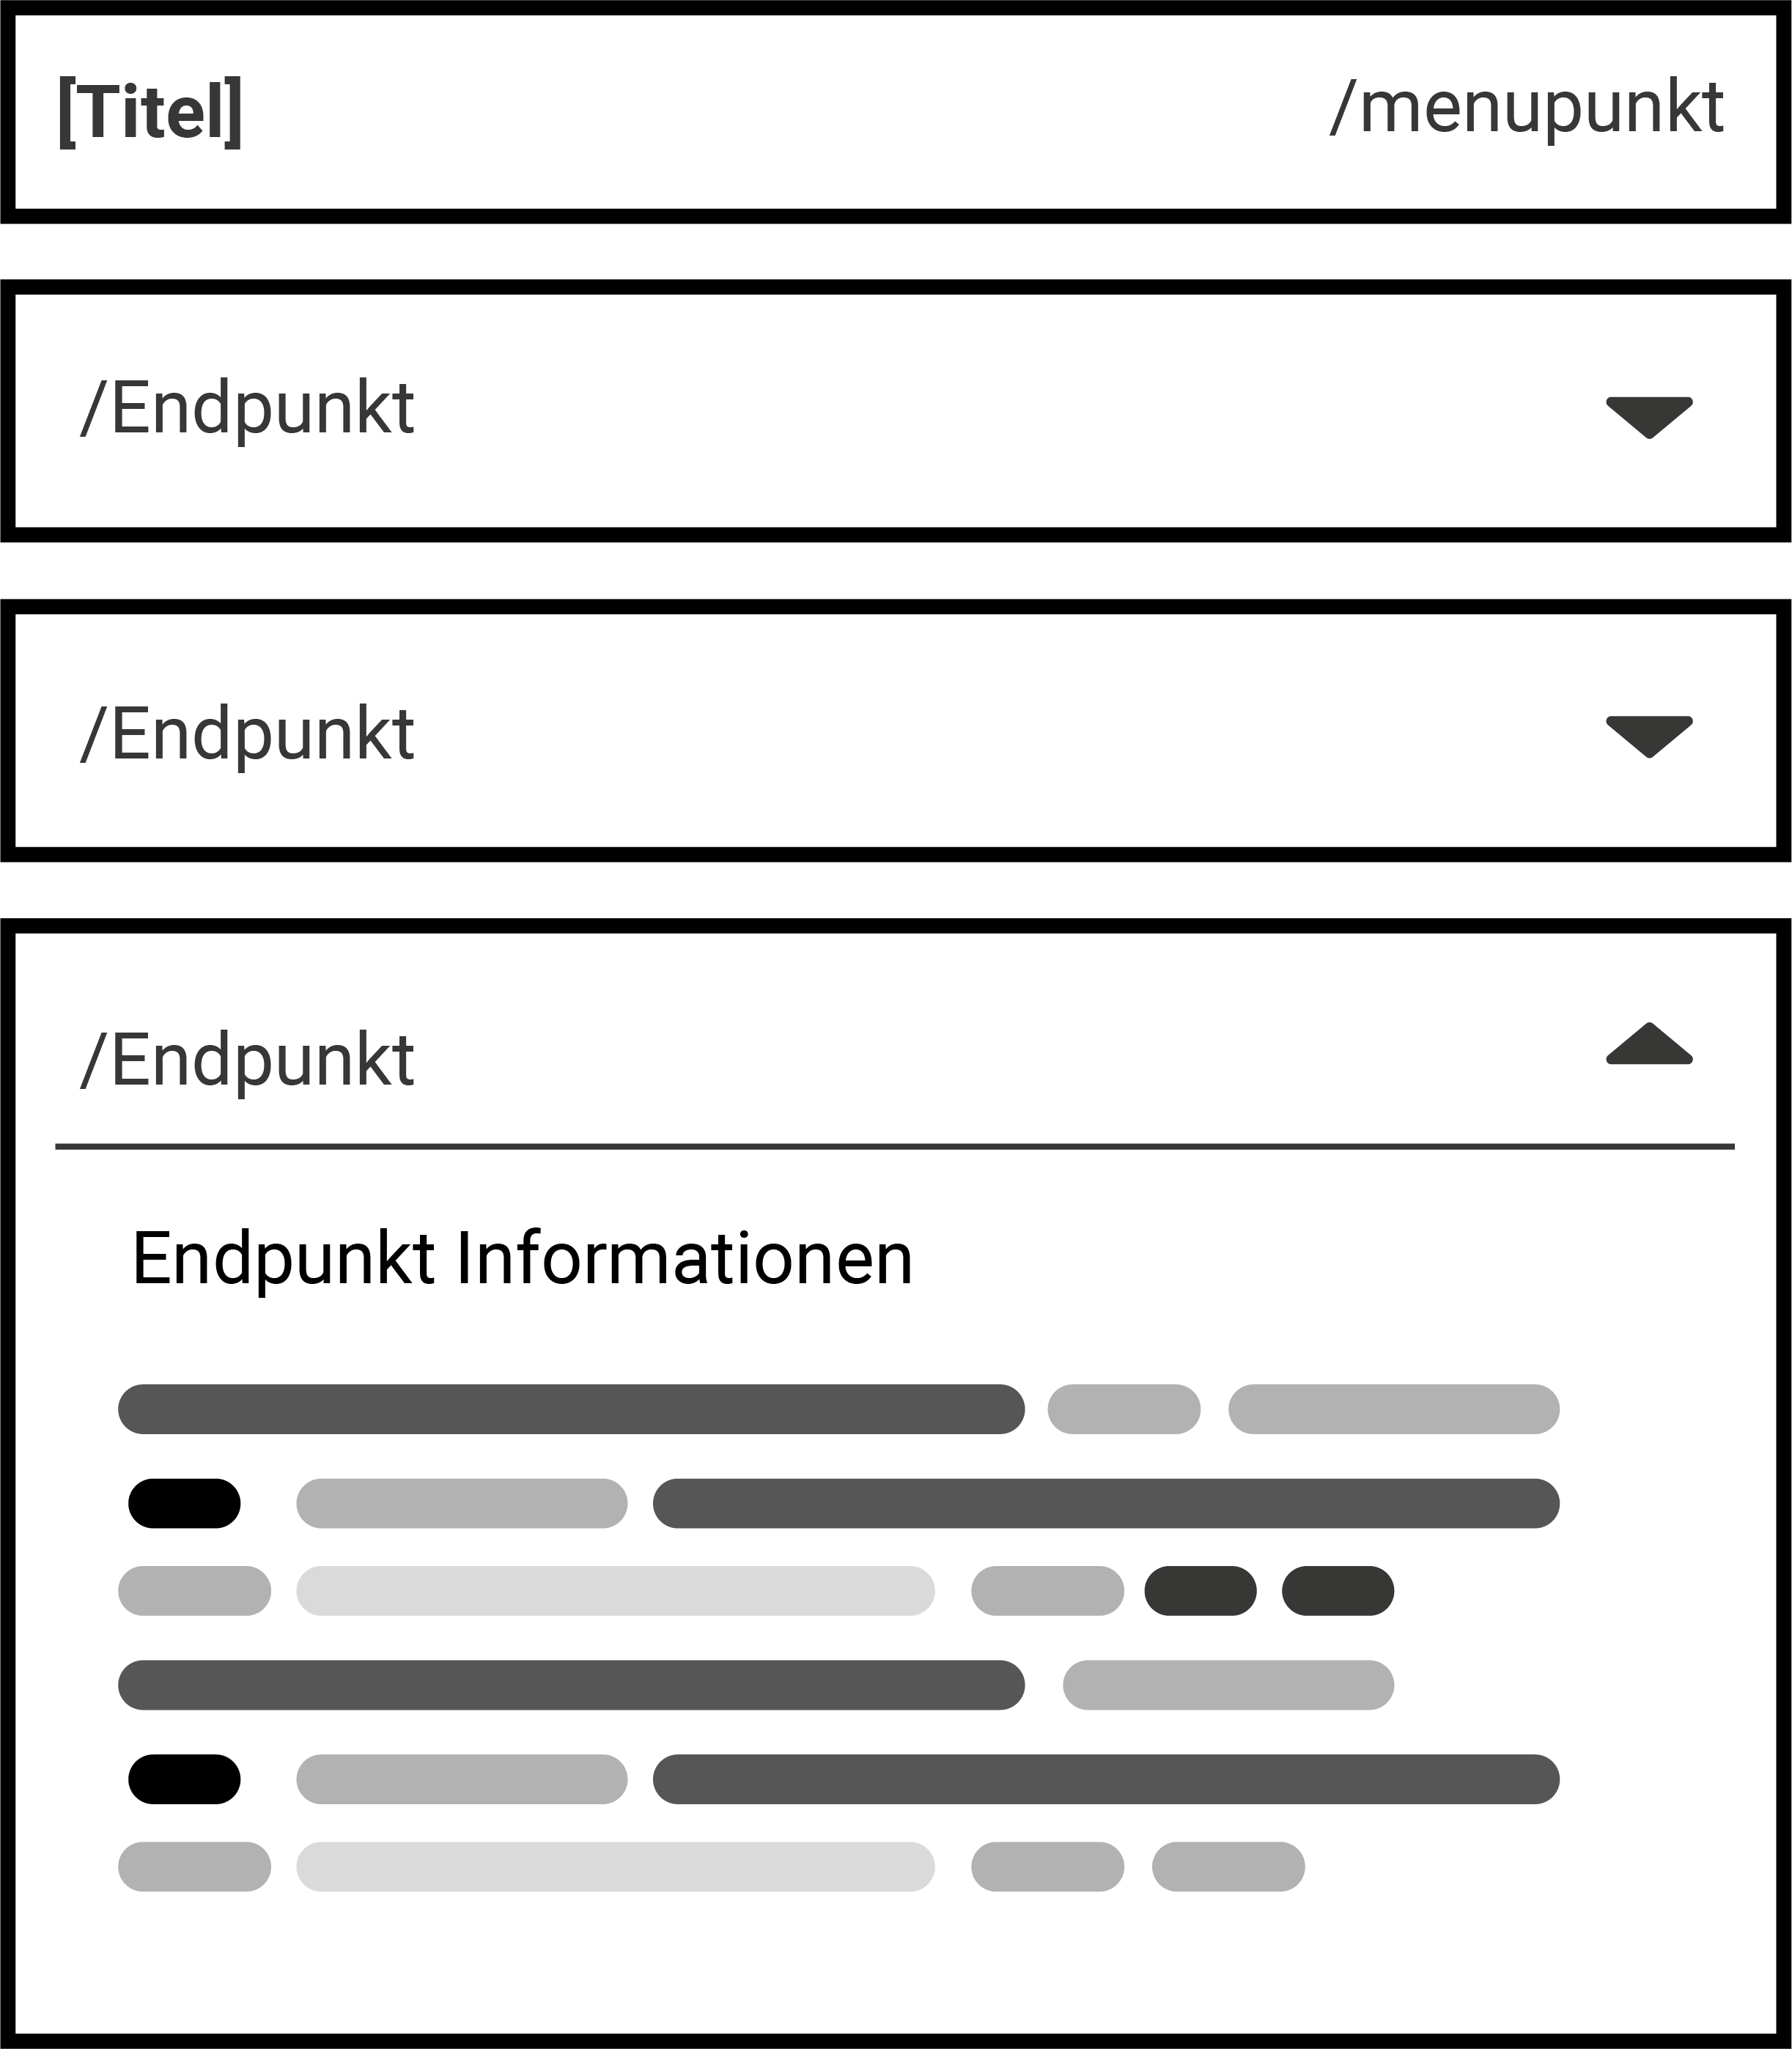
\includegraphics[width=0.6\textwidth]{figures/mock-up.png}
    \caption{Design-Prototyp}
    \label{fig:mock-up}
\end{figure}

\section{Backend} \label{sec:backend}

\subsection{Express.js}
Das sehr bekannte Framework \textit{express.js} wird verwendet, um Endpunkte der \gls{restapi} bereitzustellen. Auch das im nächsten Kapitel zu entwickelnde Frontend kann mittels dieses Frameworks bereitgestellt werden. Es bietet einige rubuste Module für die Entwicklung von Webapplikationen. In dem Buch \textit{REST API Development with Node.js} wird ein Generator verwendet, welcher das initiale Aufsetzen des Projektes und der Ordnerstrukturen stark vereinfacht. Der sogenannte \textit{express-generator} füllt ein leeres Projekt mit Ordnern, Dateien und beispielhaftem Code \cite{Doglio.2018}. Auf diesen Generator wird jedoch verzichtet, um die Entwicklung des Projektes genauer Untersuchen zu können und selbst die geeignete Ordnerstruktur anzulegen. 

Die Struktur wurde bereits im Kapitel \ref{subsub:system-architectuere} festgelegt. Auf dieser aufbauend werden die einzelnen Komponenten im Folgendem näher betrachtet.


\subsection{Controller}
Controller werden in diesem Projekt verwendet, um eingehende \gls{http}-Anfragen zu validieren und die \gls{http}-Schicht von der Business-Logik zu trennen. Wenn eingehende Anfragen nicht im richtigen Format vorliegen werden sie an dieser Stelle direkt mit einem entsprechenden Status-Code und eine Mitteilung beantwortet. 

\begin{figure}[h]
    \centering
    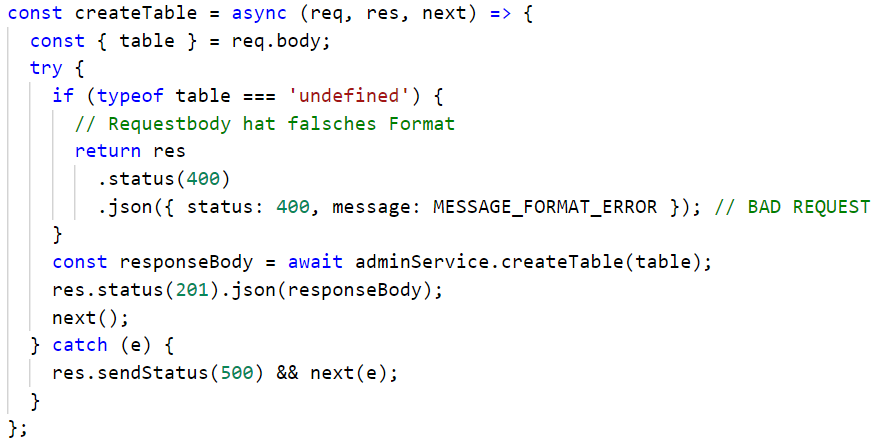
\includegraphics[width=0.8\textwidth]{figures/code-controller.png}
    \caption{createTable Methode des Admin-Controllers}
    \label{fig:createTable-controller}
\end{figure}

In der Abbildung \ref{fig:createTable-controller} lässt sich eine solche Prüfung erkennen. Zunächst wird mit
\begin{verbatim}
    const { table } = req.body;
\end{verbatim}
aus dem, in der Anfrage übergebenem, \gls{json}-Body das Objekt \textit{table} ausgelesen. im nächsten Schritt wird dann geprüft, ob dieses Objekt definiert ist. Im Negativfall wird direkt eine Antwort mit dem Status-Code 400 generiert. Dieser steht für \textit{BAD REQUEST}; also fehlerhafte Anfrage. Ist das Objekt \textit{table} jedoch definiert, wird es zur weiteren Verarbeitung an die Business-Logik weitergereicht. 
\subsection{Services}
Im Ordner \textit{Services} befindet sich die Business-Logik. Eingehende Anfragen werden aufbereitet, an die Datenbank gesendet und im \gls{json}-Format wieder an die \textit{Controller}-Schicht zurückgegeben. 

\begin{figure}[h]
    \centering
    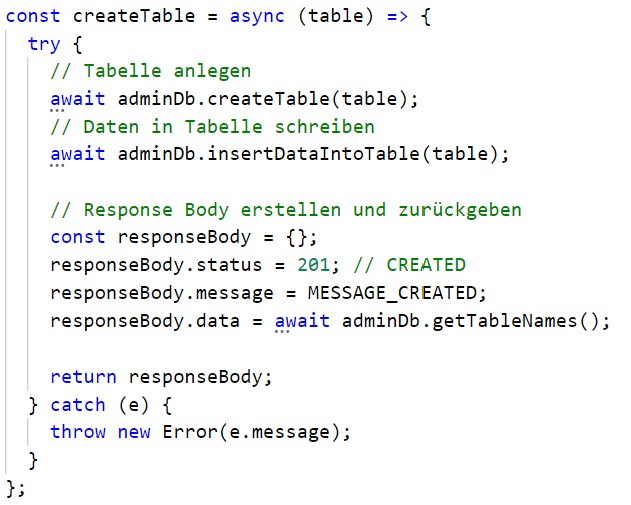
\includegraphics[width=0.6\textwidth]{figures/code-services.png}
    \caption{createTable Methode des Admin-Services}
    \label{fig:createTable-services}
\end{figure}

In Abbildung \ref{fig:createTable-services} wird das vorherige Beispiel zum Erstellen einer Tabelle wieder aufgegriffen. Die Funktion nimmt eine Tabelle im folgenden Format entgegen:

\begin{verbatim}
    {
        table: {
            name: "Tabellenname (Pfadname)",
            header: ["Erster Spaltenname", "Zweiter Spaltenname"....],
            data: [
                ["Erste Reihe 1", "Erste Reihe 2"....],
                ["Zweite Reihe 1", "Zweite Reihe 2"....]
            ]
        }
    }
\end{verbatim}

Diese Struktur wird nicht weiter verändert und über die Modul-Methode \textit{adminDb.createTable(table)} respektive \textit{adminDb.insertDataIntoTable(table)} an die nächste Schicht weitergegeben. Nach erfolgreicher Ausführung wird eine Antwort generiert. Hierzu wird ein neues Objekt erstellt: \textit{responseBody}. Diesem Objekt werden Attribute hinzugefügt.

\begin{itemize}
    \item responseBody.status: Der zurückzugebene Status-Code (in diesem Fall 201 CREATED)
    \item responseBody.message: Eine textuelle Nachricht um anzuzeigen, dass die Ressource erfolgreich erstellt wurde.
    \item responseBody.data: Hier werden noch einmal von der Model-Ebene alle Tabellennamen abgerufen, um sie mit der \gls{json}-Formatierten Antwort an die Controller-Ebene zurückzugeben. 
\end{itemize}

\subsection{Model}
Im Modul \textit{DB} (in diesem Ffalle das Datenmodell) findet die Kommunikation mit der zugrundeliegende \textit{sqlite}-Datenbank statt. Anfragen aus der Services-Schicht werden entgegengenommen, verarbeitet und beantwortet. Um das Beispiel \textit{createTable} weiterhin zu verfolgen, werden aus diesem Modul drei verschiedene Methoden vorgestellt. 

\begin{figure}[h]
    \centering
    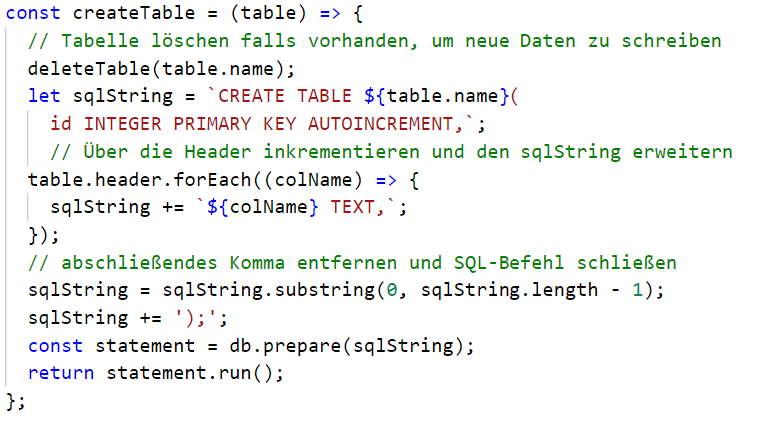
\includegraphics[width=0.8\textwidth]{figures/code-model-createTable.png}
    \caption{createTable Methode des Admin-Models}
    \label{fig:createTable-model-createTable}
\end{figure}

Die \textit{createTable}-Methode in Abbildung \ref{fig:createTable-model-createTable} nimmt ein Objekt im schon bekannten Format entgegen. Eine eventuell bestehende Tabelle wird zunächst entfernt. Dadurch kann diese Funktion auch genutzt werden, um änderungen in die Datenbank zu schreiben. 

\begin{figure}[h]
    \centering
    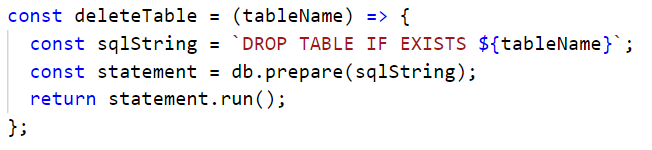
\includegraphics[width=0.8\textwidth]{figures/code-model-deleteTable.png}
    \caption{deleteTable Methode des Admin-Models}
    \label{fig:createTable-model-deleteTable}
\end{figure}

Diese Funktion ist in Abbildung \ref{fig:createTable-model-deleteTable} zu sehen und ist eine Ummantelung des \gls{sql}-Statements \textit{DROP TABLE IF EXISTS tabellenname} \cite{Gerner.2006}.


\begin{figure}[h]
    \centering
    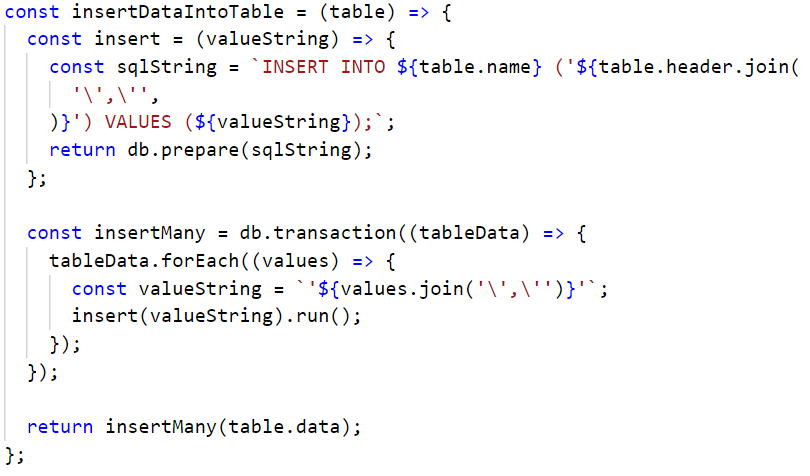
\includegraphics[width=0.8\textwidth]{figures/code-model-insertDataIntoTable.png}
    \caption{insertDataIntoTable Methode des Admin-Models}
    \label{fig:createTable-model-insertDataIntoTable}
\end{figure}

Etwas komplexer dagegen ist die Funktion \textit{insertDataIntoTable} (Abbildung \ref{fig:createTable-model-insertDataIntoTable}), welche ebenfalls das Objekt \textit{table} entgegennimmt. Diese Funktion besteht aus zwei Unterfunktionen.
Die Unterfunktionen \textit{insert} wird für jede anzulegende Tabellen-Zeile von insertMany aufgerufen. Hier wird ein \gls{sql}-Statement geformt \cite{Gerner.2006}:
\begin{verbatim}
    INSERT INTO tabellenname ('Spaltenname 1', 'Spaltenname 2'....) 
    VALUES ('Wert 1 Zeile n', 'Wert 2 Zeile n'....);
\end{verbatim}

Nach der Formung wird die gebildete Zeichenkette mit der \textit{.run()} Funktion auf der Datenbank ausgeführt. Dieser Vorgang wird so oft wiederholt, wie Zeilen mit übergeben wurden.

\subsection{Routes, Konstanten und app.js}
In diesem Unterkapitel werden die kleineren Module behandelt. Das Modul \textit{Routes} beinhaltet alle Endpunkte des Systems; sowohl die der Konfigurationsoberfläche als auch die generischen Endpunkte des Clients. Wie in Abbildung \ref{fig:routes} zu Erkennen, wird bei den Client-Routen der Platzhalter * genutzt. Somit wird hier jeder Aufruf der \gls{url}
\begin{verbatim}
    https://localhost:3000/api/
\end{verbatim}
abgefangen und verarbeitet. Auch Suchanfragen, sogenannte \textit{search querys}, werden hier berücksichtigt. Das Auslesen und Formatieren der Anfragen geschieht auf den unteren Ebenen (Controller, Services). 
\begin{figure}[h]
    \centering
    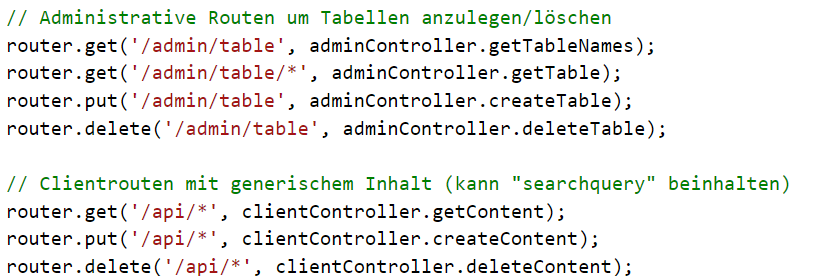
\includegraphics[width=0.8\textwidth]{figures/code-routes.png}
    \caption{Alle Routen des Systems}
    \label{fig:routes}
\end{figure}

Standard-Nachrichten, Ports und der App-Name werden im Modul \textit{Constants} aufbewahrt, somit sind diese global an jeder Stelle des Projekts verfügbar.
\\
Eine weitere wichtige Schlüsseldatei bildet die \textit{app.js}. In dieser Datei wird der \textit{express.js}-Server gestartet und mit den eben angeführtem Routen verbunden. Auch die statische Bereitstellung des Frontends  wird hier ausgeführt. Dies wird im Folgenden Kapitel näher beschrieben.

\section{Frontend} \label{sec:frontend}

\subsection{Bereitstellung und Modularisierung}

Das Frontend (die Benutzeroberfläche) mit der die lokale  \gls{restapi} angepasst wird ist eine reguläre Webseite, welche auf das Backend über die administrativen \gls{api} Schnittstellen zugreift. Die Ordner-Struktur ist relativ simpel gehalten. So gibt es einen Wurzelordner in dem sich die Hauptseite befindet (index.html) und drei Unterordner - \textit{css}, \textit{js} und \textit{assets}. 

Der Ordner \textit{js} beinhaltet JavaScript Dateien, welche die Modularisierung und die Kommunikation mit dem Backend übernehmen. In dessen Unterordner modules befinden sich Module, welche zur Laufzeit geladen werden. Dieses Prinzip ist ein relativ neues JavaScript-Feature und wird von allen modernen Browsern nativ unterstützt.

Durch die Modularisierung müssen nicht mehr alle Code-Teile eines Projekts in einer Datei gespeichert werden, 
sondern werden dynamisch importiert wenn nötig. \cite{Mozilla.2020}

Die Module sind wie folgt unterteilt:

\begin{itemize}
    \item \textit{api.js}: In diesem Modul findet ausschließlich die Kommunikation mit dem Backend statt. Die administrativen Endpunkte, welche vorher ausgearbeitet wurden, werden hier angesprochen.
    \item \textit{components.js}: Dieses Modul beherbergt Komponenten, welche dynamisch geladen und mit übergebenen Werten ausgefüllt werden. Dies verspricht einen hohe Wiederverwendbarkeit einzelner Komponenten. So wird beispielsweise eine Eintragskomponente je nach Tabelle mit den verschiedenen Hinweisen ausgefüllt. (Beschreibung der Endpunkte) 
    \item \textit{constants.js}: Hier werden nur Konstanten gespeichert welche innerhalb der Oberfläche benötigt werden, wie Endpunktmethoden, Port oder die \gls{url} des Backends.
    \item \textit{handler.js}: Diese Komponente ist für jede User-Interaktion auf der Oberfläche zuständig. Sie füllt Tabellen oder reagiert auf Knopfdrücke. Auch die Modals werden hier geladen und mit Fehler- oder Erfolgsmeldungen bestückt.
    \item \textit{util.js}: in \textit{util.js} sind Funktionen untergebracht, welche andere Funktionen unterstützen. Konvertierungen sind ein solcher Anwendungsfall. Dies wird benötigt, um zum Beispiel eine reguläre \gls{html}-Tabelle in das von der API benötigte \gls{json}-Format umzuwandeln.
\end{itemize}


Die Bereitstellung der Konfigurationsoberfläche erfolgt über den schon vorhandenen Webserver, welcher über \textit{express.js} ausgeführt wird. Erreichbar ist die Seite über einen Webbrowser unter der Adresse:

\begin{verbatim}
    http://localhost:3000
\end{verbatim}

In der Konsole wird hierzu eine entsprechende Nachricht mit dem Link ausgegeben.

\subsubsection{BEM: Block Element Modifier}
Die Anpassung der Website wird mit Hilfe von \gls{css} durchgeführt. Es gibt verschiedene Arten zur Strukturierung einer solchen Datei. Eine Möglichkeit ist die Strukturierung nach dem \gls{bem} Prinzip. Die Idee hinter dieser Namensgebung ist jedes zu stilisierende Element in bestimmte Kategorien aufzuteilen \cite{VsevolodStrukchinsky.2020, Finelli.October2017}:

\begin{itemize}
    \item Block: Elemente die für sich selbst stehen wie z.B.  \textit{header}, \textit{container}, \textit{menu} oder \textit{input}
    \item Element: Entität die nicht für sich selbst steht aber fest an einen Block gebunden ist wie z.B: \textit{header-title} oder \textit{menu-item}
    \item Modifier: Diese Attribute ändern die Erscheinung einzelner Elemente wie Farbe oder Größe z.B. \textit{color-dark}, \textit{size-m}
\end{itemize}

\section{Bündelung in Applikation} \label{sec:bundle}

Um die Applikation für verschiedene Betriebssysteme bereitzustellen, die Quelldateien möglichst in ausführbare Dateien gebündelt werden.
Idealerweise wird hierbei die Umgebung \textit{node.js} 
direkt mit eingeschlossen, um komplizierte Installationsvorgäng zu vermeiden.

Das populärste Werkzeug ist das über \gls{npm} installierbare Werkzeug \textit{pkg}. Dieses Programm erzeugt automatisch die gewünschten ausführbaren Dateien, sodass nur noch der Ordner mit den Modulen und der mit den statischen Dateien der Konfigurationsoberfläche ausgeliefert werden müssen. Der Quellcode des Backends, sowie eine aktuelle  node.js-Version werden in die ausführbaren Dateien eingebunden. \cite{igorklopov.2020}
\\
Jedoch sind bei der Benutzung in der Praxis Probleme aufgetreten. Da proprietärer Code zur Benutzung der Datenbank auf dem jeweiligen System (welches pkg ausführt) compiliert wird, ist dieser nicht mehr mit anderen Betriebssystemen kompatibel. Das heißt also ein Paket, welches unter MacOS gepackt wurde, lässt sich auch nur unter MacOS ausführen. 

Dies kann umgangen werden durch die Kompilierung auf unterschiedlichen Systemen, sodass drei verschiedene Versionen entstehen; für Windows, für Linux und eine für MacOS.


 KOMPILIERUNG BESCHREIBEN? 


\chapter{Handbuch: Benutzung des Programms} \label{chp:handbook}


\section{Konfigurationsoberfläche}
\subsection{Anzeigen und ändern eines Endpunktes}
Nach dem Aufrufen der Administrationsoberfläche, sind entweder vorhandene Tabellen gelistet oder es wird, bei nichtvorhandensein von Tabellen, nur die Kopfleiste angezeigt. 

In \autoref{fig:hb_1} ist bereits ein Endpunkt zu sehen: \textit{artikel}. 

\begin{figure}[h]
    \centering
    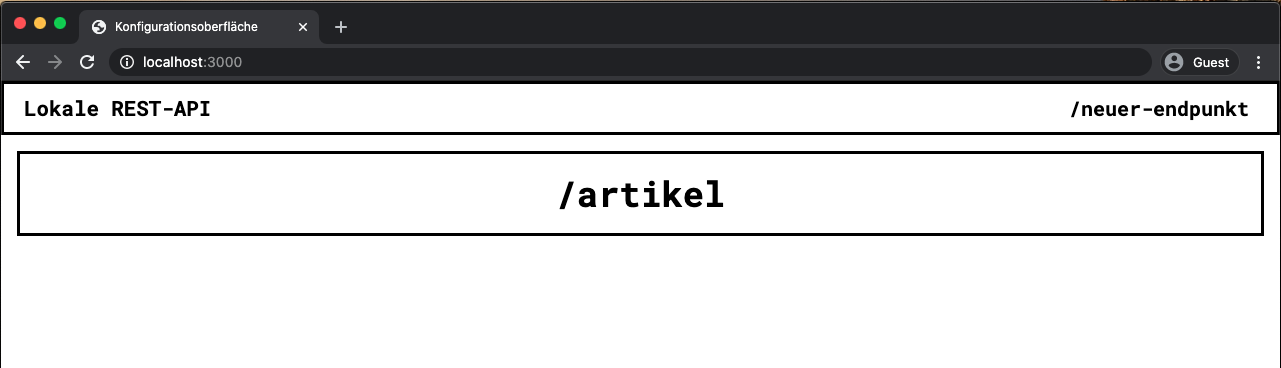
\includegraphics[width=15cm]{figures/hb_1.png}    %0.6\textwidth
    \caption{Startbildschirm der Administrationsoberfläche}
    \label{fig:hb_1}
\end{figure}

Mit einem Klick auf diesen Endpunkt wird eine Übersicht über die Benutzung angezeigt. Die verschiedene Spalten geben Auskunft über die zu verwendende Methode und dem Pfad. Zudem gibt es eine Spalte \textit{Beschreibung} in der noch einmal beschrieben wird wie die jeweilige Methode zu nutzen ist. Eine genaue Erklärung zur Nutzung der \gls{api} erfolgt im \autoref{chp:conclusion}.

\begin{figure}[H]
    \centering
    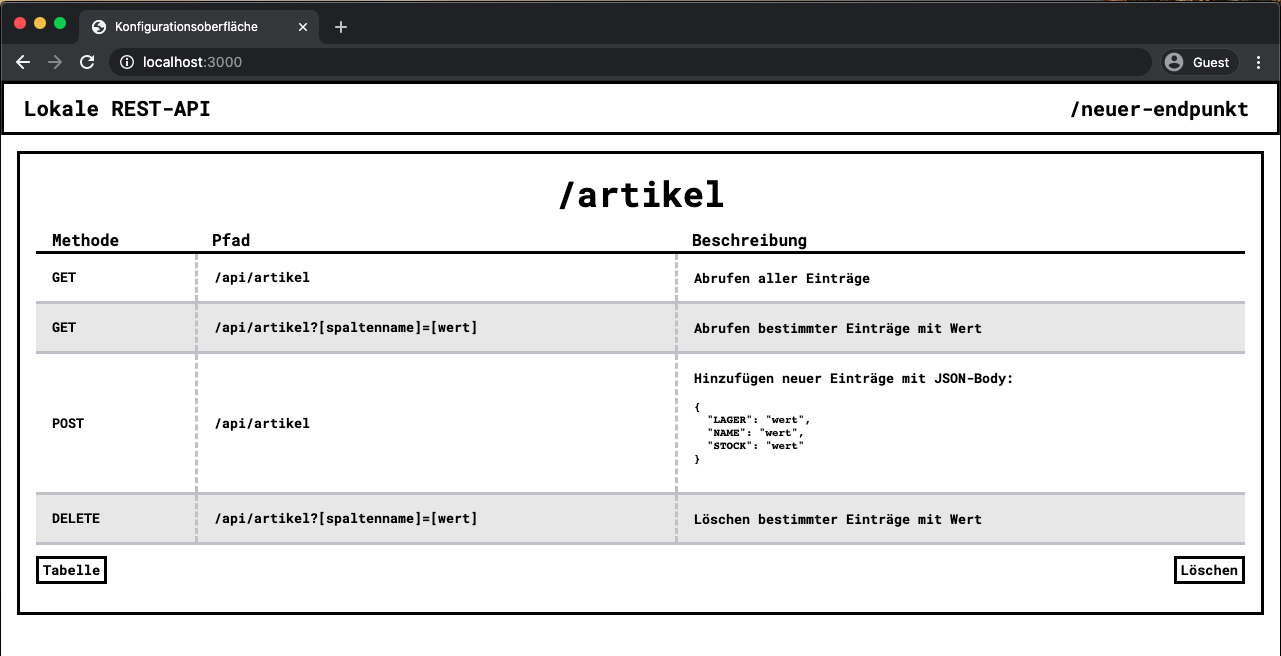
\includegraphics[width=15cm]{figures/hb_2.png}    %0.6\textwidth
    \caption{Anzeige eines Endpunktes}
    \label{fig:hb_2}
\end{figure}

Mit einem Klick auf den Button \textit{Tabelle}, öffnet sich ein Modal in dem die dazugehörigen Daten stehen (\autoref{fig:hb_3}). Oben links lässt sich die Form der Tabelle einsehen - in diesem Fall 4 Spalten und 4 Zeilen. Durch ändern der Zahlen können hier beliebig Zeilen hinzugefügt oder entfernt werden. 

\begin{figure}[H]
    \centering
    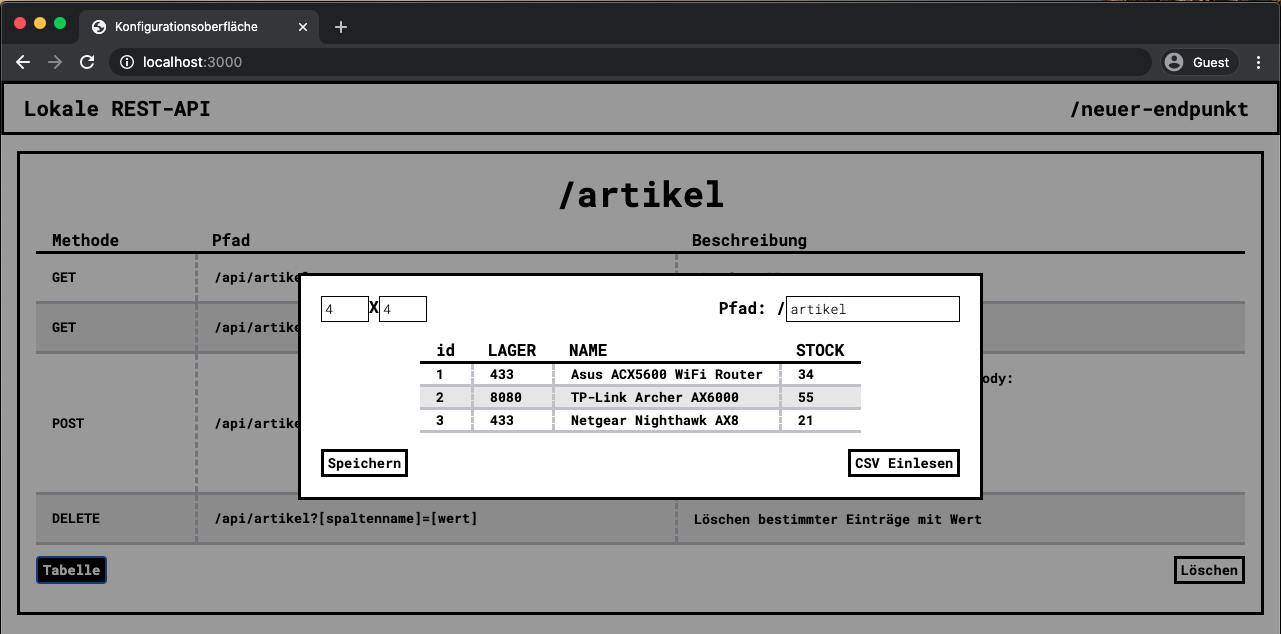
\includegraphics[width=15cm]{figures/hb_3.png}    %0.6\textwidth
    \caption{Änderung eines bestehenden Endpunktes}
    \label{fig:hb_3}
\end{figure}

Die Tabelle ist beschreibbar, was bedeutet, dass Daten durch überschreiben geändert werden können. Um gewünschte Änderungen abschließend zu persistieren, ist eine Bestätigung durch drücken des \textit{Speichern} Knopfes erforderlich.

\subsection{Erstellung eines neuen Endpunktes}

Um einen neuen Endpunkt anzulegen, wird über den Menüpunkt \textit{neuer-endpunkt} ein Modal geöffnet. Es sind mehrere Möglichkeiten zum Erstellen verfügbar. Die erste ist die manuelle Eingabe: 
Hierzu wird zunächst das Format der Datentabelle festgelegt, der Pfad des Endpunktes angegeben und anschließend Daten in die Tabelle eingetragen. Eine eindeutige ID ist nicht nötigt, da diese automatisch bei Speicherung der Tabelle erzeugt wird. Nach erfolgreicher Erstellung wird die Startübersicht inklusive der neu erstellten Tabelle angezeigt. 

\begin{figure}[H]
    \centering
    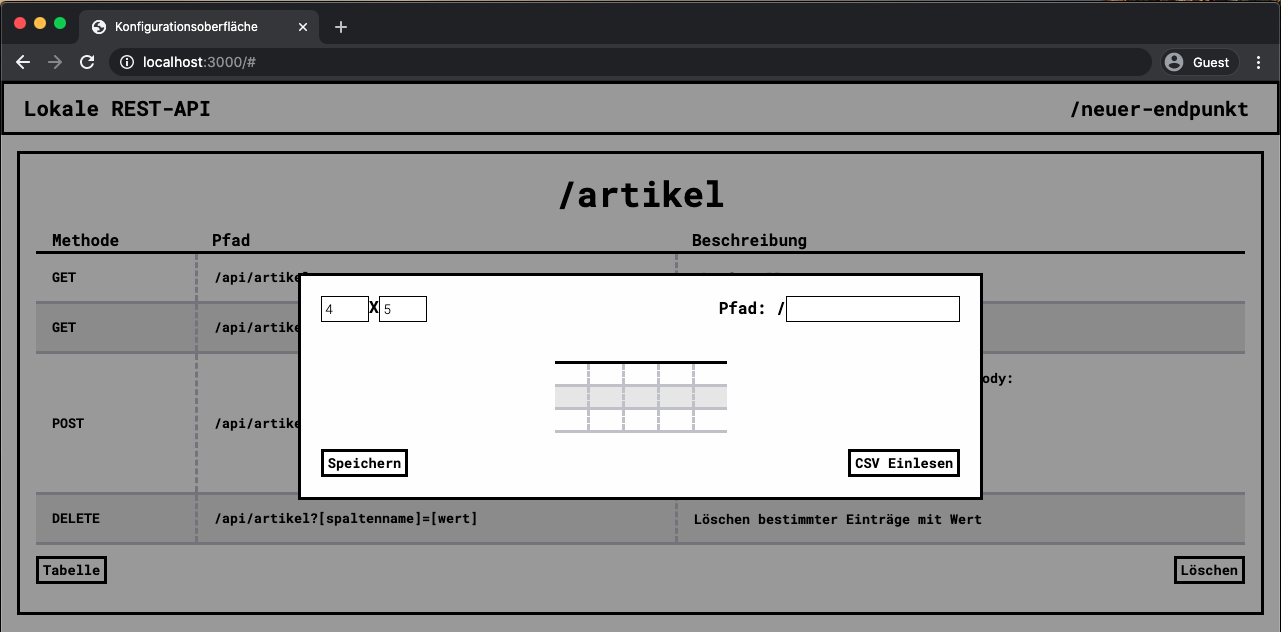
\includegraphics[width=15cm]{figures/hb_4.png}    %0.6\textwidth
    \caption{Anlegen eines neuen Endpunktes}
    \label{fig:hb_4}
\end{figure}
Weiterhin ist es möglich eine \gls{csv}-Datei einzulesen. Das einzuhaltende Format ist in \autoref{fig:hb_5} abgebildet. Die erste Zeile ist immer die Kopfzeile der Tabelle. Spalten werden durch Kommata voneinander abgegrenzt und eine neue Zeile wird durch einen Zeilenumbruch gekennzeichnet. 

\begin{figure}[H]
    \centering
    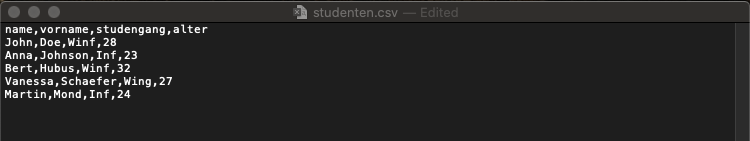
\includegraphics[width=15cm]{figures/hb_5.png}    %0.6\textwidth
    \caption{Format einer CSV-Datei}
    \label{fig:hb_5}
\end{figure}

Durch das Bestätigen der Schaltfläche \textit{CSV Einlesen} erscheint ein Dateidialog, wie in \autoref{fig:hb_6} zu sehen. Durch die Auswahl der entsprechenden Datei, wird diese eingelesen. 
\begin{figure}[H]
    \centering
    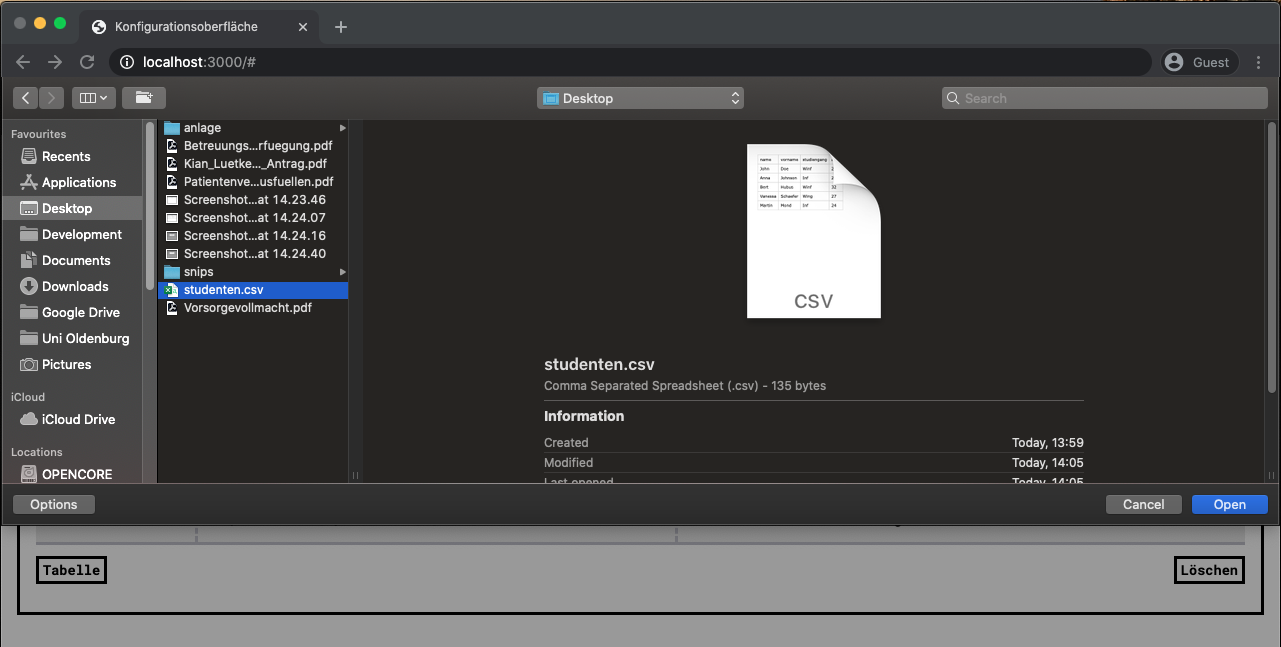
\includegraphics[width=15cm]{figures/hb_6.png}    %0.6\textwidth
    \caption{Einlesen einer CSV-Datei}
    \label{fig:hb_6}
\end{figure}

Nach erfolgreichem Hochladen der \gls{csv}-Datei erscheinen die Daten in einem neuen Modal. Hier besteht die Möglichkeit Änderungen vorzunehmen. Zudem muss der gewünschte Pfad (Name des Endpunktes) angegeben werden.

\begin{figure}[H]
    \centering
    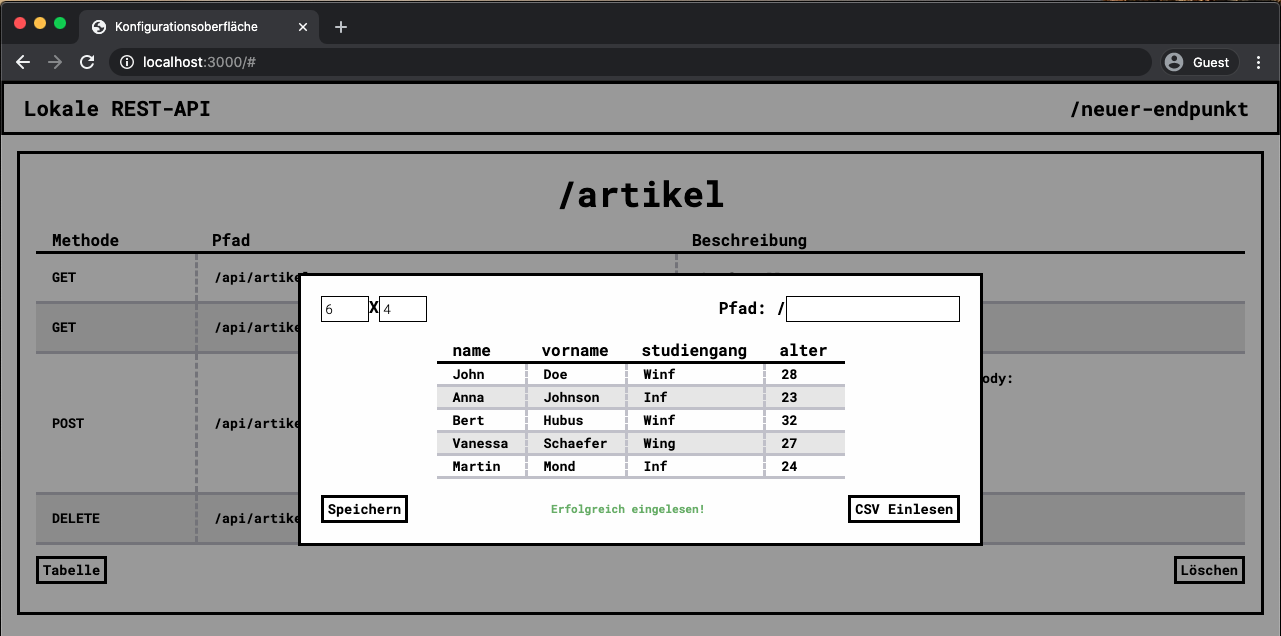
\includegraphics[width=15cm]{figures/hb_7.png}    %0.6\textwidth
    \caption{Anzeige der importierten Tabelle}
    \label{fig:hb_7}
\end{figure}

\newpage
\section{REST-API}

\subsection{Datenabfrage}

Um die erstellten Endpunkte abzufragen, müssen \gls{http}-Requests auf die entsprechende \gls{url} ausgeführt werden. Die einfachste Form ist das Konsolen Programm \textit{curl}. Dieses gehört bei den meisten Betriebssystemen zum Standard und ist auch unter dem hier verwendeten MacOS Teil des Systems \cite{DanielStenbergandContributers.2020}.

\begin{verbatim}
> curl localhost:3000/api/artikel | json_pp
{
   "message" : "Request successful",
   "status" : 200,
   "data" : [
      {
         "STOCK" : "34",
         "NAME" : "Asus ACX5600 WiFi Router",
         "LAGER" : "433",
         "id" : 1
      },
      {
         "LAGER" : "8080",
         "NAME" : "TP-Link Archer AX6000",
         "STOCK" : "55",
         "id" : 2
      },
      [...]
   ]
}
\end{verbatim}

Der obige Ausschnitt zeigt, wie ein einfacher GET-Request auf den Endpunkt \textit{artikel} ausgeführt wird.
Durch die Übergabe an das ebenfalls standardmäßig vorhandene Konsolenprogramm \textit{json\_pp} wird die Ausgabe ansprechender formatiert. Dies ist nicht zwingend notwendig, verbessert jedoch die Übersichtlichkeit. Die Ausgabe zeigt eine Nachricht, dass die Anfrage Fehlerfrei war, sowie den Status-Code 200. Zudem wird das Array \textit{data} zurückgegeben, welches die angeforderten Daten enthält.

Um nun nur einen bestimmten Artikel auszugeben wird ein querystring an den GET-Request angehängt:
\begin{verbatim}
> curl http://localhost:3000/api/artikel\?id\=1 |json_pp                                                                                                                                       
{
   "status" : 200,
   "message" : "Request successful",
   "data" : [
      {
         "LAGER" : "433",
         "NAME" : "Asus ACX5600 WiFi Router",
         "id" : 1,
         "STOCK" : "34"
      }
   ]
}
\end{verbatim}

Hervorzuheben ist, dass bei der Benutzung von \textit{curl} Ssonderzeichen, wie zum Beispiel das ? oder das \& Zeichen ein vorgestelltes / Zeichen benötigen, damit die Abfrage korrekt funktioniert. 

\subsection{Datenmanipulation: Erstellen und Löschen}
Um einen neuen Eintrag der Tabelle hinzuzufügen bedarf es eines POST-Requests. Dies beherrscht das Werkzeug \textit{curl} ebenfalls. Folgendes Listing illustriert ein solches Vorgehen:

\begin{verbatim}
> curl -d '{"LAGER": "433", "NAME": "Huawei AX3 Standard", "STOCK": "4"}' \
-H "Content-Type: application/json" \
-X POST http://localhost:3000/api/artikel | json_pp 
{
   "message" : "Ressource successfully created",
   "status" : 201,
   "data" : [
         [...]
         {
            "STOCK" : "4",
            "id" : 5,
            "LAGER" : "433",
            "NAME" : "Huawei AX3 Standard"
         }
      ]
}
\end{verbatim}

Dabei werden einige Parameter genutzt:
\begin{itemize}
    \item \textit{-d}: das d steht für data, hier wird der \gls{json}-Body übergeben. 
    \item \textit{-H}: An dieser stelle können \gls{http}-Header übergeben werden.
    \item \textit{-X}: Dieser Buchstabe steht für den Request-Typ; in diesem Fall POST.
\end{itemize}

Wie in diesem Beispiel zu sehen Antwortet die \gls{api} nicht nur mit einer Erfolgsmeldung, sondern gibt auch alle Daten zurück inklusive der neu hinzugefügten.

Schließlich fehlt noch das Löschen vorhandener Einträge. Dafür wird der \gls{http}-Request DELETE genutzt, wie folgendes Listing veranschaulicht:
\newpage
\begin{verbatim}
> curl -X DELETE http://localhost:3000/api/artikel\?id\=2 | json_pp
{
   "status" : 200,
   "data" : [
      {
         "STOCK" : "21",
         "id" : 3,
         "LAGER" : "433",
         "NAME" : "Netgear Nighthawk AX8"
      },
      {
         "NAME" : "Huawei AX3 PRO",
         "STOCK" : "12",
         "LAGER" : "433",
         "id" : 4
      },
      {
         "NAME" : "Huawei AX3 Standard",
         "LAGER" : "433",
         "id" : 5,
         "STOCK" : "4"
      }
   ],
   "message" : "Request successful"
}
\end{verbatim}

Hier lässt sich erkennen, dass wieder der -X Parameter genutzt wurde, um die Methode DELETE auszuwählen. Die \gls{api} gibt eine Erfolgsmeldung zurück  sowie die verbleibenden Daten der Tabelle.
\include{sections/conclusion}
}

\pagenumbering{Roman}
\setcounter{page}{\thesavepage}

\appendix
\include{sections/appendix}

\addcontentsline{toc}{chapter}{Literaturverzeichnis}
\bibliographystyle{alpha}
\bibliography{bibliography} % Point to BibTeX literature file e.g. literatur.bib

\include{sections/affidavit}

\end{document}